\documentclass[13pt]{extarticle}

\usepackage{amsmath}
\usepackage{amssymb}
\usepackage{amsthm}
\usepackage[a4paper,margin=2.3cm]{geometry}
\usepackage{xcolor}
\usepackage{graphicx}
\usepackage{enumitem}
\usepackage{titlesec}
\usepackage[most]{tcolorbox}
\usepackage{colortbl}
\usepackage{array}
\usepackage{listings}
\usepackage{hyperref}
\hypersetup{colorlinks=true,linkcolor=blue,urlcolor=blue}

\usepackage{xepersian}
\settextfont{Vazirmatn FD}
\setmonofont{Menlo}[Scale=0.80]

\setlength{\emergencystretch}{3em}
\hyphenpenalty=10000
\exhyphenpenalty=10000

\definecolor{headblue}{RGB}{200,90,140}
\definecolor{boxbg}{RGB}{252,240,246}
\definecolor{claimbg}{RGB}{250,235,243}
\definecolor{proofaccent}{RGB}{225,180,200}

% ---- code colors ----
\definecolor{codebg}{RGB}{250,247,251}
\definecolor{codekw}{RGB}{175,55,110}
\definecolor{codecmt}{RGB}{120,125,135}
\definecolor{codestr}{RGB}{45,120,85}
\definecolor{codenum}{RGB}{180,180,190}

% ---- section / subsection styling ----
\titleformat{\section}
  {\Large\bfseries\color{headblue}}{\thesection}{0.6em}{}
  [{\vspace{2pt}\color{headblue!35}\titlerule[1.2pt]}]
\titlespacing*{\section}{0pt}{0pt}{12pt}
\titleformat{\subsection}
  {\large\bfseries\color{headblue!88}}{\thesubsection}{0.5em}{}
\titlespacing*{\subsection}{0pt}{10pt}{6pt}

% ---- note box ----
\newtcolorbox{notex}{
  breakable, enhanced, boxrule=0pt, arc=3pt,
  colback=claimbg, frame hidden,
  borderline east={3pt}{0pt}{headblue},
  left=10pt, right=12pt, top=7pt, bottom=7pt,
}

% ---- python listing style ----
\lstdefinestyle{py}{
  language=Python,
  basicstyle=\ttfamily\footnotesize,
  keywordstyle=\color{codekw}\bfseries,
  commentstyle=\color{codecmt}\itshape,
  stringstyle=\color{codestr},
  numbers=left,
  numberstyle=\tiny\color{codenum},
  numbersep=8pt,
  backgroundcolor=\color{codebg},
  frame=single,
  framesep=5pt,
  rulecolor=\color{proofaccent},
  breaklines=true,
  showstringspaces=false,
  columns=fullflexible,
  keepspaces=true,
  xleftmargin=14pt,
  aboveskip=8pt,
  belowskip=8pt,
}
\newenvironment{pycode}{\begin{latin}\lstset{style=py}}{\end{latin}}

% ---- console-output style ----
\lstdefinestyle{out}{
  basicstyle=\ttfamily\scriptsize\color{black!82},
  backgroundcolor=\color{black!5},
  frame=leftline,
  framesep=6pt,
  rulecolor=\color{headblue!55},
  linewidth=\linewidth,
  breaklines=true,
  columns=fullflexible,
  keepspaces=true,
  xleftmargin=12pt,
  aboveskip=6pt,
  belowskip=8pt,
}
\newenvironment{consoleout}{\par\smallskip\begin{latin}\lstset{style=out}}{\end{latin}}

% ---- "linked to question" box ----
\newtcolorbox{qlink}{
  breakable, enhanced, boxrule=0pt, arc=3pt,
  colback=boxbg, frame hidden,
  borderline west={3pt}{0pt}{headblue!70},
  left=10pt, right=12pt, top=6pt, bottom=6pt,
  before upper={\textbf{\color{headblue}پاسخِ عددیِ پرسش.}\enspace}
}

\newcommand{\R}{\mathbb{R}}
\newcommand{\norm}[1]{\left\lVert #1 \right\rVert}
\newcommand{\T}{^{\top}}
\newcommand{\file}[1]{\lr{\texttt{#1}}}

\begin{document}

\noindent{\small\textbf{ملیکا زارع}\quad\textbar\quad شماره دانشجویی: ۴۰۱۱۳۴۱۶\quad\textbar\quad{\color{black!65} جبر خطی عددی --- تمرین سری چهارم --- توضیح کد و تحلیل خروجی}}
\vspace{4pt}
{\color{headblue!40}\hrule height 1pt}
\vspace{10pt}

%==================================================================
\section{ساختار کلی پروژه}
%==================================================================

هدفِ کلیِ الگوریتم، تقسیمِ یک تصویر به چند ناحیه‌ی همگن است. برای این منظور تصویر را به‌صورتِ یک گراف مدل می‌کنیم که در آن هر پیکسل یک گره است و پیکسل‌های شبیه و نزدیک با یالی سنگین به هم متصل می‌شوند. سپس با استفاده از مقادیر و بردارهای ویژه‌ی لاپلاسینِ این گراف، مرزهای کم‌هزینه‌ی برش شناسایی و تصویر از همان نقاط قطعه‌بندی می‌شود. برای خوانایی و ماژولار بودنِ پیاده‌سازی، این مسیر به هشت فایلِ مستقل تقسیم شده است؛ هر فایل یک گام از زنجیره را انجام می‌دهد و فایلِ \file{run\_all.py} همه را به‌ترتیب اجرا کرده و شکل‌های خروجی را در پوشه‌ی \file{outputs/} ذخیره می‌کند.

\smallskip
\noindent\textbf{روندِ کلیِ داده در خط‌لوله:} تصویر $\rightarrow$ ویژگی‌های هر پیکسل ($X,F$) $\rightarrow$ ماتریسِ تشابهِ $W$ $\rightarrow$ لاپلاسینِ $L_{\mathrm{sym}}$ $\rightarrow$ بردارهای ویژه‌ی کوچک ($z_2,\dots,z_k$) $\rightarrow$ خوشه‌بندیِ \lr{k-means} $\rightarrow$ برچسبِ هر پیکسل (تصویرِ قطعه‌بندی‌شده). ورودیِ هر گام، خروجیِ گامِ پیش از آن است.

\begin{center}
\renewcommand{\arraystretch}{1.35}
\arrayrulecolor{headblue!40}
\setlength{\arrayrulewidth}{0.8pt}
\begin{tabular}{|l|l|}
\hline
\rowcolor{headblue}
{\color{white}\textbf{فایل}} & {\color{white}\textbf{وظیفه}} \\ \hline
\rowcolor{boxbg}\file{step1\_image.py}     & بارگذاری تصویر و ساختِ بردارهای ویژگی (مکان و روشنایی) \\ \hline
\file{step2\_weights.py}   & ساختِ ماتریسِ تشابهِ متقارنِ $W$ (پرسش ۱) \\ \hline
\rowcolor{boxbg}\file{step3\_laplacian.py} & ساختِ لاپلاسینِ نرمال‌شده $L_{\mathrm{sym}}$ و بررسیِ طیف (پرسش ۲) \\ \hline
\file{step5\_plu.py}       & تجزیه‌ی $PLU$ و حلِ دستگاه مثلثی از پایه (پرسش ۵) \\ \hline
\rowcolor{boxbg}\file{step4\_deflation.py} & توانِ معکوس $+$ حذف برای یافتنِ بردارهای فیدلر (پرسش ۳ و ۴) \\ \hline
\file{step6\_segmentation.py} & \lr{k-means} دستی و قطعه‌بندی برای $k=2,3,4$ (پرسش ۶) \\ \hline
\rowcolor{boxbg}\file{step7\_lanczos.py}  & لانتساش روی ماتریسِ تُنُکِ تصویرِ بزرگ (پرسش ۷) \\ \hline
\file{step8\_zebra.py}     & اجرای همان خط‌لوله روی تصویرِ واقعیِ گورخر (نمونه‌ی مقایسه) \\ \hline
\end{tabular}
\arrayrulecolor{black}
\end{center}

%==================================================================
\section{گام ۱ --- بارگذاری تصویر و ساخت ویژگی‌ها}
%==================================================================

معیارِ شباهتِ دو پیکسل بر دو عامل استوار است: میزانِ هم‌رنگی و میزانِ نزدیکیِ مکانی. بنابراین برای هر پیکسل دو ویژگی نگه می‌داریم: مختصاتِ مکانی‌اش $X_i=(row,col)$ و شدتِ روشنایی‌اش $F_i$. برای آنکه بتوان درستیِ الگوریتم را به‌سادگی ارزیابی کرد، به‌جای یک تصویرِ واقعی ابتدا یک تصویرِ مصنوعیِ ساده تولید می‌شود: تابعِ \file{make\_synthetic\_image} یک دیسکِ روشن (شدت $\approx0.85$) را در مرکزِ یک زمینه‌ی تیره (شدت $\approx0.15$) قرار می‌دهد و نویزِ گاوسیِ کوچکی به آن می‌افزاید. از آنجا که پاسخِ درست (تفکیکِ دایره از زمینه) از پیش معلوم است، صحّتِ خروجی به‌سادگی قابلِ داوری است.

\smallskip
\noindent\textbf{روندِ کد.} تصویر یک آرایه‌ی دوبعدیِ $H\times W$ است، اما برای کار با گراف لازم است هر پیکسل به‌صورتِ یک سطر بازنمایی شود. تابعِ \file{build\_features} این تبدیل را انجام می‌دهد: نخست با \file{reshape} تصویر را به شکلی درمی‌آورد که هر پیکسل یک سطر از ماتریسِ روشناییِ $F$ باشد (در نتیجه $n=H\cdot W$ سطر خواهیم داشت)؛ سپس با \file{np.mgrid} شماره‌ی سطر و ستونِ هر پیکسل را می‌سازد و آن‌ها را در ماتریسِ مکانِ $X$ می‌چیند. خروجیِ این تابع، همین دو ماتریسِ $X$ و $F$ است که ورودیِ گامِ بعد (ساختِ ماتریسِ تشابه) خواهند بود.

\begin{pycode}
\begin{lstlisting}
def build_features(img):
    # X: pixel coords (n, 2), F: intensities (n, c)
    H, W = img.shape[:2]
    F = img.reshape(H * W, -1)                 # each pixel -> one feature row
    rows, cols = np.mgrid[0:H, 0:W]
    X = np.stack([rows.ravel(), cols.ravel()], axis=1).astype(float)
    return X, F, (H, W)
\end{lstlisting}
\end{pycode}

\noindent\textbf{خروجیِ اجرا:}
\begin{consoleout}
\begin{lstlisting}
image (50, 50) -> n = 2500 pixels, X (2500, 2), F (2500, 1)
intensity range: [0.072, 0.902]
\end{lstlisting}
\end{consoleout}

\noindent یعنی تصویرِ $50\times50$ به $n=2500$ گره تبدیل شد، ماتریسِ مکان $X$ ابعادِ $(2500,2)$ و ماتریسِ روشنایی $F$ ابعادِ $(2500,1)$ دارد. بازه‌ی شدت $[0.072,\,0.902]$ است --- کف و سقف حولِ همان $0.15$ و $0.85$ به‌علاوه‌ی نویز، که نشان می‌دهد تصویر درست ساخته شده است.

\begin{center}
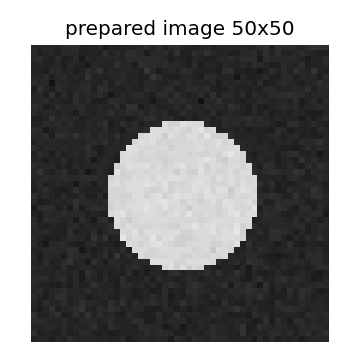
\includegraphics[width=0.34\linewidth]{../Q4-CODE/outputs/step1_image.png}\\[3pt]
{\small خروجیِ تصویریِ گام ۱: دیسکِ روشن روی زمینه‌ی تیره ($50\times50$).}
\end{center}

%==================================================================
\section{گام ۲ --- ماتریس تشابه $W$ (پرسش ۱)}
%==================================================================

پس از استخراجِ ویژگی‌ها، گراف ساخته می‌شود. برای هر جفت پیکسل یک وزن تعریف می‌کنیم که میزانِ شباهتِ آن‌ها را نشان می‌دهد: هرچه دو پیکسل هم‌رنگ‌تر و نزدیک‌تر باشند وزن بزرگ‌تر است، و با افزایشِ اختلافِ روشنایی یا فاصله، وزن به‌سرعت کاهش می‌یابد. یک ملاحظه‌ی کارایی نیز در نظر گرفته شده است: ارتباطِ هر پیکسل با پیکسل‌های بسیار دور اهمیتی ندارد، بنابراین برای هر جفت که فاصله‌ی مکانی‌شان از شعاعِ $r$ بیشتر باشد وزن را صفر قرار می‌دهیم. در نتیجه بیشترِ درایه‌های $W$ صفر می‌شوند (ماتریس \emph{تُنُک} می‌شود) و در حافظه و زمانِ محاسبات صرفه‌جویی چشمگیری حاصل می‌شود.

\begin{pycode}
\begin{lstlisting}
def build_weight_matrix(X, F, sigma_I=0.1, sigma_X=4.0, r=5.0, dense=True):
    sqX = np.sum(X ** 2, axis=1)
    dX2 = sqX[:, None] + sqX[None, :] - 2.0 * (X @ X.T)
    sqF = np.sum(F ** 2, axis=1)
    dF2 = sqF[:, None] + sqF[None, :] - 2.0 * (F @ F.T)
    np.clip(dX2, 0.0, None, out=dX2)          # rounding can make tiny negatives

    W = np.exp(-dF2 / sigma_I ** 2) * np.exp(-dX2 / sigma_X ** 2)
    W[dX2 >= r ** 2] = 0.0                      # keep only neighbors within r
    np.fill_diagonal(W, 0.0)                    # W_ii = 0
    return W if dense else sp.csr_matrix(W)
\end{lstlisting}
\end{pycode}

\noindent\textbf{روندِ کد.} محاسبه‌ی مستقیمِ فاصله‌ها با دو حلقه‌ی تودرتو برای $n=2500$ گره به میلیون‌ها عملیات می‌انجامد و بسیار کُند است. به‌جای آن از محاسبه‌ی برداری استفاده می‌کنیم: با اتحادِ $\norm{a-b}^2=\norm{a}^2+\norm{b}^2-2a\cdot b$ می‌توان تمامِ فاصله‌های دوبه‌دو را یک‌جا و با ضربِ ماتریسی به‌دست آورد. بدین‌ترتیب کد نخست \file{dX2} (مربعِ فاصله‌های مکانی) و \file{dF2} (مربعِ فاصله‌های روشنایی) را می‌سازد و سپس دو کرنلِ گاوسی را در هم ضرب می‌کند تا $W$ حاصل شود. سه نکته‌ی پیاده‌سازی که در کد لحاظ شده است:
\begin{itemize}[leftmargin=1.6em,itemsep=1pt,topsep=2pt]
\item گاهی بر اثرِ خطای گِرد‌کردن، مربعِ فاصله مقداری منفیِ بسیار کوچک می‌شود (که از نظرِ ریاضی ناممکن است)؛ \file{clip} این مقادیر را به صفر می‌بُرد تا جذر و تابعِ نمایی دچار خطا نشوند.
\item خطِ \file{W[dX2 >= r**2] = 0} شرطِ همسایگی را اعمال می‌کند: هر جفت با فاصله‌ی بیش از $r$ صفر می‌شود. این خط عاملِ اصلیِ تُنُک ماندنِ $W$ است.
\item \file{np.fill\_diagonal(W, 0)} قطر را صفر می‌کند، زیرا هیچ پیکسلی با خودش یال ندارد ($W_{ii}=0$).
\end{itemize}
شایانِ ذکر است که تقارنِ $W$ به‌صورتِ ذاتی برقرار است و نیازی به تحمیلِ آن نیست: چون \file{dX2} و \file{dF2} از رابطه‌ای متقارن نسبت به $i$ و $j$ ساخته شده‌اند، $W_{ij}$ و $W_{ji}$ یکسان به‌دست می‌آیند --- همان نتیجه‌ای که در پرسشِ ۱ به‌صورتِ تحلیلی اثبات شد.

\begin{pycode}
\begin{lstlisting}
def symmetry_error(W):
    return float(np.linalg.norm(W - W.T, ord="fro"))   # ||W - W^T||_F
\end{lstlisting}
\end{pycode}

\noindent\textbf{خروجیِ اجرا:}
\begin{consoleout}
\begin{lstlisting}
params: sigma_I=0.1, sigma_X=4.0, r=5.0
W shape : (2500, 2500), range [0.0000, 0.9394]
max|diag|: 0.00e+00
nonzeros: 2.51%
||W - W^T||_F = 0.000e+00
\end{lstlisting}
\end{consoleout}

\begin{qlink}
\textbf{پرسش ۱-ب} می‌خواست تقارنِ $W$ را \emph{عددی} تأیید کنیم. تابعِ \file{symmetry\_error} کمیتِ $\norm{W-W\T}_F$ را حساب می‌کند و خروجی دقیقاً $\mathbf{0.000\times10^{0}}$ شد. یعنی نه‌فقط تقریباً، بلکه \emph{بیت‌به‌بیت} $W_{ij}=W_{ji}$؛ این تأییدِ عملیِ همان اثباتِ تحلیلی است. همچنین بیشینه‌ی قطر $=0$ (قرارداد $W_{ii}=0$ رعایت شده) و فقط $\mathbf{2.51\%}$ درایه‌ها ناصفرند، یعنی ماتریس به‌شدت تُنُک است.
\end{qlink}

\noindent نمودارِ زیر (\file{step2\_W\_spy.png}) این تُنُکی را به‌صورتِ یک نوارِ باریکِ قطری نشان می‌دهد: هر پیکسل فقط با همسایه‌های نزدیکش (که در ترتیبِ سطری-ستونیِ تصویر شماره‌های نزدیک دارند) پیوند دارد و بقیه‌ی ماتریس صفر است.

\begin{center}
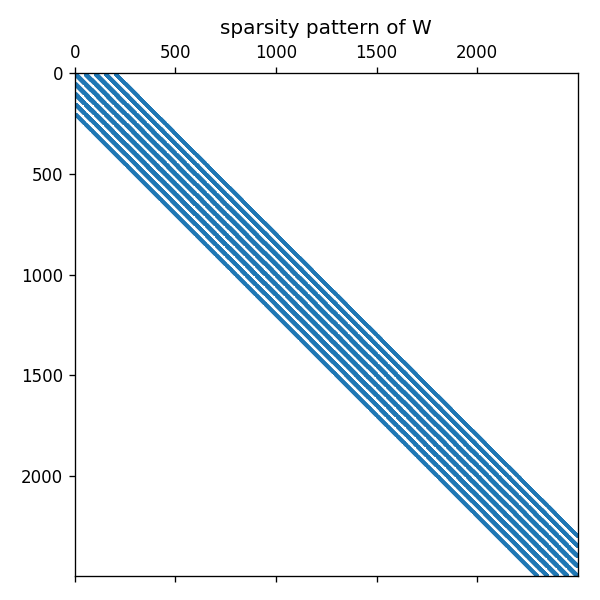
\includegraphics[width=0.46\linewidth]{../Q4-CODE/outputs/step2_W_spy.png}\\[3pt]
{\small خروجیِ تصویریِ گام ۲: الگوی تُنُکیِ $W$؛ فقط یک نوارِ باریکِ قطری ناصفر است.}
\end{center}

%==================================================================
\section{گام ۳ --- لاپلاسین نرمال‌شده (پرسش ۲)}
%==================================================================

ماتریسِ $W$ به‌تنهایی برای برش کافی نیست و باید نرمال‌سازی شود تا گره‌های پُرارتباط به‌طورِ نامتناسب غالب نشوند. ابتدا درجه‌ی هر گره ($d_i=\sum_j W_{ij}$، یعنی مجموعِ وزنِ یال‌هایش) محاسبه و سپس لاپلاسینِ نرمال‌شده‌ی $L_{\mathrm{sym}}=I-D^{-1/2}WD^{-1/2}$ ساخته می‌شود. تمامِ خواصی که در پرسشِ ۲ اثبات شد (تقارن، قرارگیریِ طیف در $[0,2]$ و بردارِ ویژه‌ی بدیهیِ صفر) مربوط به همین ماتریس است، و بردارهای ویژه‌ی کوچکِ آن همان مؤلفه‌هایی هستند که در گام‌های بعد برای برش به کار می‌روند.

\begin{pycode}
\begin{lstlisting}
def build_normalized_laplacian(W):
    W = np.asarray(W, dtype=float)
    n = W.shape[0]
    d = W.sum(axis=1)
    d_inv_sqrt = 1.0 / np.sqrt(np.where(d > 0, d, 1.0))   # guard isolated nodes
    L = np.eye(n) - d_inv_sqrt[:, None] * W * d_inv_sqrt[None, :]
    L = 0.5 * (L + L.T)                                    # enforce exact symmetry
    return L, d, d_inv_sqrt
\end{lstlisting}
\end{pycode}

\noindent\textbf{روندِ کد.} کد گام‌به‌گام همان فرمول را می‌سازد. ابتدا با \file{W.sum(axis=1)} درجه‌ی همه‌ی گره‌ها یک‌جا محاسبه می‌شود. سپس به‌جای ساختِ کاملِ ماتریسِ قطریِ $D^{-1/2}$ (که کم‌بار و پُرهزینه است)، تنها بردارِ $d\_inv\_sqrt$ نگه‌داری و با یک ضربِ سطری/ستونی اثرِ آن روی $W$ اعمال می‌شود؛ نتیجه یکسان اما بسیار کم‌هزینه‌تر است. دو محافظِ عددی نیز در نظر گرفته شده است: (۱) برای گره‌های منزوی که درجه‌ی صفر دارند، به‌جای تقسیم بر صفر مقدارِ $1$ قرار داده می‌شود؛ (۲) خطِ \file{L = 0.5*(L + L.T)} تقارن را به‌صورتِ صریح تضمین می‌کند، زیرا خطاهای کوچکِ ممیزِ شناور می‌توانند تقارنِ تحلیلی را اندکی مخدوش کنند.

\smallskip
\noindent تابعِ \file{spectral\_report} بخشی از الگوریتمِ اصلی نیست و صرفاً برای راستی‌آزمایی افزوده شده است: با استفاده از تابعِ \file{eigh}، ادعاهای تئوریِ پرسشِ ۲ به‌صورتِ عددی سنجیده می‌شوند تا اطمینان حاصل شود که خروجیِ کد با نتایجِ اثبات‌شده مطابقت دارد:

\begin{pycode}
\begin{lstlisting}
evals, evecs = np.linalg.eigh(L)      # reference spectrum (verification only)
v = np.sqrt(d); v /= np.linalg.norm(v)          # trivial eigenvector D^{1/2} 1
Lv = L @ v
"min_eig": evals.min(), "max_eig": evals.max(),
"in_0_2": evals.min() >= -1e-8 and evals.max() <= 2 + 1e-8,
"trivial_residual": np.linalg.norm(Lv),         # ||L (D^{1/2} 1)||
"trivial_rayleigh": v @ Lv,                      # v^T L v
"num_near_zero": int(np.sum(evals < 1e-6)),
\end{lstlisting}
\end{pycode}

\noindent\textbf{خروجیِ اجرا:}
\begin{consoleout}
\begin{lstlisting}
L_sym shape : (2500, 2500), ||L - L^T||_F = 0.000e+00
eig range = [-3.270764e-16, 1.096398e+00], all in [0, 2]? True
||L * (D^1/2 1)|| = 1.913e-16, Rayleigh = 2.754e-19
num near-zero eig = 2
trivial in bottom subspace = 1.000000
\end{lstlisting}
\end{consoleout}

\begin{qlink}
\textbf{پرسش ۲-الف (تقارن).} خروجیِ $\norm{L-L\T}_F=\mathbf{0}$ نشان می‌دهد $L_{\mathrm{sym}}$ دقیقاً متقارن است --- تأییدِ عددیِ همان اثباتِ $L_{\mathrm{sym}}\T=L_{\mathrm{sym}}$.

\smallskip
\textbf{پرسش ۲-ب (طیف در $[0,2]$).} کوچک‌ترین مقدار ویژه $\approx-3.3\times10^{-16}$ (عملاً صفر و فقط خطای ماشین) و بزرگ‌ترین $\approx\mathbf{1.096}$؛ پرچمِ \lr{\texttt{in\_0\_2}} برابرِ \lr{True} شد. یعنی کلِ طیف داخلِ بازه‌ی تئوریِ $[0,2]$ نشست.

\smallskip
\textbf{پرسش ۲-ج (بردارِ بدیهیِ صفر).} باقی‌مانده‌ی $\norm{L\,(D^{1/2}\mathbf 1)}=\mathbf{1.9\times10^{-16}}$ و خارج‌قسمتِ رِیلیِ $v\T L v=\mathbf{2.8\times10^{-19}}$ (هر دو $\approx 0$) عملاً معادله‌ی $L_{\mathrm{sym}}(D^{1/2}\mathbf 1)=\mathbf 0$ را تأیید می‌کنند؛ پس $D^{1/2}\mathbf 1$ واقعاً بردارِ ویژه‌ی مقدار ویژه‌ی صفر است.
\end{qlink}

\noindent مشاهده‌ی درخورِ توجه آن است که تعدادِ مقادیر ویژه‌ی نزدیکِ صفر برابرِ $\mathbf 2$ به‌دست آمد. این نشان می‌دهد که با این پارامترها، دیسک و زمینه چنان کم به هم متصل‌اند که گراف تقریباً به \emph{دو مؤلفه‌ی مجزا} تفکیک می‌شود --- که با انتظارِ اولیه (یک شیء و یک پس‌زمینه) سازگار است. در نمودارِ زیر ۲۰ مقدار ویژه‌ی کوچک ترسیم شده است؛ منحنی از صفر آغاز و به‌صورتِ پله‌ای صعود می‌کند، و محلِ جهش‌های ناگهانی (گافِ طیفی) بیانگرِ تعدادِ خوشه‌های طبیعیِ تصویر است.

\begin{center}
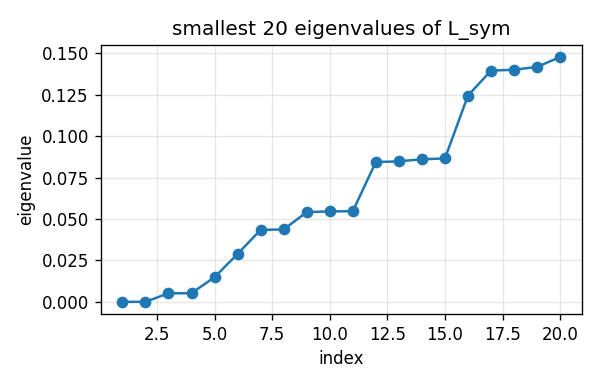
\includegraphics[width=0.62\linewidth]{../Q4-CODE/outputs/step3_eigs.png}\\[3pt]
{\small ۲۰ مقدار ویژه‌ی کوچکِ $L_{\mathrm{sym}}$؛ صعودی و آغازشونده از صفر.}
\end{center}

%==================================================================
\section{گام ۵ --- تجزیه‌ی $PLU$ از پایه (پرسش ۵)}
%==================================================================

پیش از یافتنِ بردارهای ویژه، به یک ابزارِ پایه نیاز داریم: حلِ دستگاه‌های خطی. کارِ اصلیِ روشِ توانِ معکوس، حلِ مکررِ دستگاهِ $(\mu I-L)x=b$ است. معکوس‌گیریِ کاملِ ماتریس هم پُرهزینه و هم از نظرِ عددی نامطلوب است؛ رویکردِ استانداردِ بهتر آن است که ماتریس \emph{یک‌بار} به حاصل‌ضربِ دو ماتریسِ مثلثی تجزیه شود ($PA=LU$) و پس از آن، برای هر سمتِ راست تنها دو دستگاهِ مثلثیِ ساده حل شود. چون ماتریسِ سمتِ چپ در تمامِ تکرارها ثابت است و فقط بردارِ $b$ تغییر می‌کند، این رویکرد صرفه‌جوییِ محاسباتیِ چشمگیری به‌همراه دارد.

\begin{pycode}
\begin{lstlisting}
def plu_decomposition(A):
    # Gaussian elimination with partial pivoting -> P A = L U
    U = np.array(A, dtype=float); n = U.shape[0]
    L = np.eye(n); P = np.eye(n)
    for k in range(n):
        p = k + int(np.argmax(np.abs(U[k:, k])))   # largest pivot in column k
        if p != k:
            U[[k, p], :] = U[[p, k], :]
            P[[k, p], :] = P[[p, k], :]
            L[[k, p], :k] = L[[p, k], :k]
        L[k + 1:, k] = U[k + 1:, k] / U[k, k]       # multipliers
        U[k + 1:, k:] -= np.outer(L[k + 1:, k], U[k, k:])   # eliminate below pivot
    return P, L, U
\end{lstlisting}
\end{pycode}

\noindent\textbf{روندِ کد.} این پیاده‌سازی همان حذفِ گاوسی با محورگیریِ جزئی است. کد ستون‌به‌ستون پیش می‌رود و در هر ستون: نخست با \file{argmax} بزرگ‌ترین درایه (به‌قدرِ مطلق) را می‌یابد و با تعویضِ سطر آن را روی قطر قرار می‌دهد --- این کار از تقسیم بر مقادیرِ بسیار کوچک و بروزِ ناپایداریِ عددی جلوگیری می‌کند؛ همین تعویض روی $P$ (که جابه‌جایی‌ها را ثبت می‌کند) و بخشِ ساخته‌شده‌ی $L$ نیز اعمال می‌شود. سپس ضرایبِ حذف در $L$ ذخیره و با یک به‌روزرسانیِ برداری (\file{np.outer}) تمامِ سطرهای زیرِ محور یک‌جا صفر می‌شوند. تابعِ \file{make\_plu\_solver} این تجزیه را \emph{تنها یک‌بار} انجام می‌دهد و تابعِ \file{solve} را بازمی‌گرداند که پس از آن برای هر بردارِ $b$ جدید فقط دو جای‌گذاریِ مثلثی (پیش‌رو و پس‌رو) انجام می‌دهد:

\begin{pycode}
\begin{lstlisting}
def make_plu_solver(A):
    P, L, U = plu_decomposition(A)              # factor ONCE: O(n^3)
    def solve(b):                               # each call: O(n^2)
        pb = P @ np.asarray(b, dtype=float)
        return back_substitution(U, forward_substitution(L, pb))
    return solve
\end{lstlisting}
\end{pycode}

\noindent این دقیقاً همان بهینه‌سازیِ $O(n^3)+T\cdot O(n^2)$ در برابرِ $O(T\,n^3)$ است که در پرسشِ ۵ تحلیل شد: چون ماتریسِ $(\mu I-L)$ در همه‌ی تکرارهای توانِ معکوس ثابت است، تجزیه یک‌بار انجام می‌شود و در هر تکرار فقط جای‌گذاری تکرار می‌شود.

\smallskip
\noindent\textbf{خروجیِ اجرا} (آزمونِ خودکارِ فایل روی ماتریسِ تصادفیِ $6\times6$):
\begin{consoleout}
\begin{lstlisting}
||P A - L U|| = 2.660e-16
||A x - b||   = 6.384e-16
\end{lstlisting}
\end{consoleout}

\begin{qlink}
\textbf{پرسش ۵} خواستِ درستیِ تجزیه و صرفه‌ی هزینه بود. خطای بازساختِ تجزیه $\norm{PA-LU}=\mathbf{2.7\times10^{-16}}$ و خطای حلِ دستگاه $\norm{Ax-b}=\mathbf{6.4\times10^{-16}}$ هر دو در حدِ دقتِ ماشین ($\sim10^{-16}$)‌اند؛ پس پیاده‌سازیِ دستیِ $PLU$ و جای‌گذاری‌ها هم درست و هم پایدارند و می‌توانند بی‌خطر در حلقه‌ی توانِ معکوس بازاستفاده شوند.
\end{qlink}

%==================================================================
\section{گام ۴ --- توان معکوس و حذف (پرسش ۳ و ۴)}
%==================================================================

این گام هسته‌ی اصلیِ الگوریتم است: یافتنِ بردارهای ویژه‌ی کوچک (بردارهای فیدلرِ $z_2,\dots,z_k$) که مرزهای برش را مشخص می‌کنند. روشِ به‌کار‌رفته، توانِ معکوس است که به کوچک‌ترین مقادیر ویژه همگرا می‌شود. اما یک مانع وجود دارد: کوچک‌ترین مقدار ویژه همان صفرِ بدیهی است و الگوریتم به‌طورِ طبیعی به سمتِ آن میل می‌کند. برای رفعِ این مشکل، در هر گام مؤلفه‌ی بردارهای پیشین (از جمله بردارِ بدیهی) را از بردارِ جاری حذف می‌کنیم (تصویرِ متعامد)؛ و چون خطای گِرد‌کردن این مؤلفه‌ها را به‌تدریج بازمی‌گرداند، این حذف باید در \emph{هر} تکرار تکرار شود --- همان استدلالی که در پرسشِ ۴ ارائه شد.

\begin{pycode}
\begin{lstlisting}
def inverse_power_deflation(L, mu=0.0, deflate_vectors=None, ...):
    Q = np.stack(deflate_vectors, axis=1) if deflate_vectors else np.zeros((n, 0))
    deflate = lambda x: x - Q @ (Q.T @ x) if Q.shape[1] else x   # project out
    x = deflate(...); x /= np.linalg.norm(x)
    for it in range(1, max_iter + 1):
        y = deflate(solver(x))       # solve (mu I - L) y = x, then RE-deflate
        y /= np.linalg.norm(y)
        if y @ x < 0: y = -y         # fix sign for a stable stopping test
        diff = np.linalg.norm(y - x); x = y
        lam = float(x @ (L @ x))     # Rayleigh quotient on L
        if diff < tol: return lam, x, it
    return lam, x, max_iter
\end{lstlisting}
\end{pycode}

\noindent\textbf{روندِ کد.} حلقه‌ی اصلی سرراست است: در هر تکرار دستگاهِ $(\mu I-L)y=x$ حل می‌شود (با همان \file{solver} گامِ ۵)، بردارِ $y$ نرمال و علامتش تثبیت می‌شود (تا معیارِ توقف نوسان نکند)، و هنگامی که دو تکرارِ متوالی به هم نزدیک شوند ($\norm{y-x}<\text{tol}$) حلقه پایان می‌یابد. دو بخشِ این حلقه دقیقاً پیاده‌سازیِ پرسش‌های ۳ و ۴ هستند:
\begin{itemize}[leftmargin=1.6em,itemsep=1pt,topsep=2pt]
\item \textbf{حذف (پرسش ۳):} در تحلیلِ نظری، حذفِ یک مقدار ویژه با ساختِ ماتریسِ $B=A-\lambda_1X_1X_1\T$ انجام می‌شد. در پیاده‌سازی نیازی به ساختِ صریحِ این ماتریس نیست و همان اثر با تصویرِ متعامدِ $\text{\lr{deflate}}(x)=x-Q(Q\T x)$ و با هزینه‌ی کمتر حاصل می‌شود، که مؤلفه‌ی بردارهای پیشین را از $x$ حذف می‌کند.
\item \textbf{حذفِ مکرر (پرسش ۴-ب):} خطِ کلیدی \file{y = deflate(solver(x))} است. تابعِ \file{deflate} \emph{پس از هر حل} فراخوانی می‌شود، نه تنها یک‌بار در ابتدا؛ زیرا در هر ضربِ ماتریسی، خطای گِرد‌کردن مقداری از مؤلفه‌ی بردارِ بدیهی را دوباره وارد می‌کند که باید در هر گام حذف شود.
\end{itemize}
تابعِ \file{compute\_segmentation\_eigenvectors} این مراحل را به‌صورتِ حذفِ انباشته سازمان می‌دهد: از بردارِ بدیهیِ $z_1=D^{1/2}\mathbf 1/\norm{\cdot}$ آغاز می‌کند، $z_2$ را می‌یابد و آن را به فهرستِ بردارهای حذف‌شونده می‌افزاید، سپس به سراغِ $z_3$ می‌رود و همین روند تا $z_k$ ادامه می‌یابد. افزون بر این، ماتریسِ $(\mu I-L)$ تنها یک‌بار تجزیه شده و در تمامِ این جست‌وجوها بازاستفاده می‌شود.

\smallskip
\noindent\textbf{خروجیِ اجرا} (برای $k=3$):
\begin{consoleout}
\begin{lstlisting}
eigenvalues (inverse power + deflation), k=3:
  z2: lambda = -1.281127e-18
  z3: lambda = 5.152878e-03
reference (eigh): [-3.270764e-16  8.241957e-16  5.152878e-03  5.196305e-03]
|z2 . z1(trivial)| = 1.266e-16
|z3 . z2|          = 3.095e-16
residual ||L z2 - lambda z2|| = 7.161e-13
residual ||L z3 - lambda z3|| = 4.172e-12
\end{lstlisting}
\end{consoleout}

\begin{qlink}
\textbf{پرسش ۳ (درستیِ حذف).} مقادیر ویژه‌ای که توانِ معکوس $+$ حذف پیدا کرد ($\lambda_{z_2}\approx0$ و $\lambda_{z_3}=\mathbf{5.152878\times10^{-3}}$) دقیقاً با ردیفِ مرجعِ \file{eigh} می‌خوانند (که $5.152878\times10^{-3}$ را می‌دهد). پس حذف واقعاً مقدار ویژه‌ی قبلی را برمی‌دارد و اجازه می‌دهد مقدارِ بعدی ظاهر شود --- همان ادعای $B=A-\lambda_1X_1X_1\T$.

\smallskip
\textbf{پرسش ۴-الف (تعامد).} $|z_2\!\cdot z_1|=\mathbf{1.3\times10^{-16}}$ و $|z_3\!\cdot z_2|=\mathbf{3.1\times10^{-16}}$؛ یعنی بردارهای یافته‌شده تا حدِ دقتِ ماشین بر هم و بر بردارِ بدیهی عمودند، همان‌طور که برای ماتریسِ متقارن انتظار داشتیم.

\smallskip
\textbf{پرسش ۴-ب (چرا تصویرگیریِ مکرر).} باقی‌مانده‌های $\norm{Lz_i-\lambda_i z_i}$ در حدِ $10^{-13}$--$10^{-12}$ ماندند و الگوریتم به سمتِ جوابِ بدیهی منحرف \emph{نشد}؛ این نتیجه‌ی مستقیمِ تکرارِ تصویرگیری در هر گام است.
\end{qlink}

\noindent (توجه: چون در این تصویر دو مقدار ویژه‌ی نزدیکِ صفر داریم، $z_2$ عملاً یک مُدِ دیگرِ نزدیک‌صفر است و اولین مقدار ویژه‌ی «واقعاً ناصفر» در $z_3$ ظاهر می‌شود؛ این با ستونِ مرجعِ \file{eigh} کاملاً سازگار است.)

%==================================================================
\section{گام ۶ --- k-means و قطعه‌بندی (پرسش ۶)}
%==================================================================

تا این مرحله بردارهای ویژه‌ی $z_2,\dots,z_k$ در اختیار است، اما این‌ها هنوز برچسبِ پیکسل‌ها نیستند بلکه بازنماییِ تازه‌ای از هر پیکسل به‌شمار می‌روند. بردارها را ستون‌به‌ستون کنارِ هم می‌چینیم؛ در نتیجه هر پیکسل به یک سطر تبدیل می‌شود که نقشِ «امضا» یا مختصاتِ آن پیکسل در فضای طیفی را دارد. پیکسل‌هایی که به یک ناحیه تعلق دارند، امضاهای نزدیک به هم پیدا می‌کنند و کافی است این نقاط در فضای امضاها خوشه‌بندی شوند؛ این کار با \lr{k-means} انجام می‌شود. (نکته‌ی فنی: پیش از خوشه‌بندی، امضاها با $y=D^{-1/2}z$ به فضای برشِ نرمال‌شده بازگردانده می‌شوند.) الگوریتمِ \lr{k-means} نیز از پایه پیاده‌سازی شده است: ابتدا با \lr{k-means++} مراکزِ اولیه را به‌گونه‌ای انتخاب می‌کند که از یکدیگر دور باشند (برای پایداریِ بیشترِ نتیجه)، سپس تکرارِ لُوید را اجرا می‌کند: تخصیصِ هر نقطه به نزدیک‌ترین مرکز، به‌روزرسانیِ مراکز به مرکزِ ثقلِ خوشه‌ها، و تکرارِ این روند تا همگرایی.

\begin{pycode}
\begin{lstlisting}
def kmeans(Xf, k, n_iter=100, seed=0):
    rng = np.random.default_rng(seed)
    centers = _kmeans_plusplus_init(Xf, k, rng)
    labels = np.full(Xf.shape[0], -1)
    for _ in range(n_iter):
        d2 = ((Xf[:, None, :] - centers[None, :, :]) ** 2).sum(axis=2)
        new_labels = d2.argmin(axis=1)            # assign to nearest center
        if np.array_equal(new_labels, labels): break   # converged
        labels = new_labels
        for c in range(k):                        # update centers
            mask = labels == c
            if mask.any(): centers[c] = Xf[mask].mean(axis=0)
    return labels

def segment(L, d, k, mu=1e-3):
    _, Z = compute_segmentation_eigenvectors(L, d, k=k, mu=mu)
    Y = Z / np.sqrt(d)[:, None]     # back to the Ncut embedding y = D^{-1/2} z
    return kmeans(Y, k)
\end{lstlisting}
\end{pycode}

\noindent\textbf{روندِ کد.} تابعِ \file{segment} کلِ خط‌لوله را در سه مرحله خلاصه می‌کند: بردارهای ویژه را از گامِ ۴ دریافت می‌کند ($Z$)، آن‌ها را با تقسیم بر $\sqrt d$ به فضای برشِ نرمال‌شده می‌برد ($Y$)، و $Y$ را به \lr{k-means} می‌دهد تا برچسبِ هر پیکسل حاصل شود. برای افزایشِ سرعت، بردارهای ویژه \emph{یک‌بار} برای بزرگ‌ترین $k$ محاسبه می‌شوند و برای $k=2,3,4$ تنها زیرمجموعه‌ی مناسبی از ستون‌ها به کار می‌رود، بی‌آنکه محاسبه از ابتدا تکرار شود.

\smallskip
\noindent\textbf{خروجیِ اجرا:}
\begin{consoleout}
\begin{lstlisting}
k=2: cluster sizes = [2011, 489]
k=3: cluster sizes = [993, 1018, 489]
k=4: cluster sizes = [810, 489, 620, 581]
\end{lstlisting}
\end{consoleout}

\begin{qlink}
\textbf{پرسش ۶} خواستِ تحلیلِ نتایجِ قطعه‌بندی بود. اندازه‌ی خوشه‌ها را عددی بخوانیم: در $k=2$ یک خوشه‌ی $\mathbf{489}$تایی (دقیقاً دیسک، $\approx$ مساحتِ دایره‌ی شعاعِ $12.5$ روی شبکه‌ی $50\times50$) از زمینه‌ی $2011$تایی جدا می‌شود. در $k=3$ همان خوشه‌ی $\mathbf{489}$تایی دست‌نخورده می‌ماند و فقط زمینه به دو تکه‌ی $993$ و $1018$ می‌شکند. در $k=4$ باز هم $\mathbf{489}$ ثابت است و زمینه به سه تکه ($810,620,581$) خرد می‌شود.

\smallskip
عددِ کلیدی این است که خوشه‌ی $\mathbf{489}$ در هر سه $k$ تغییر نمی‌کند: یعنی «شیء» یک واحدِ پایدار است و افزایشِ $k$ فقط پس‌زمینه را ریزتر می‌کند. این همان ادعای گزارش است که با اعداد تأیید می‌شود.
\end{qlink}

\begin{center}
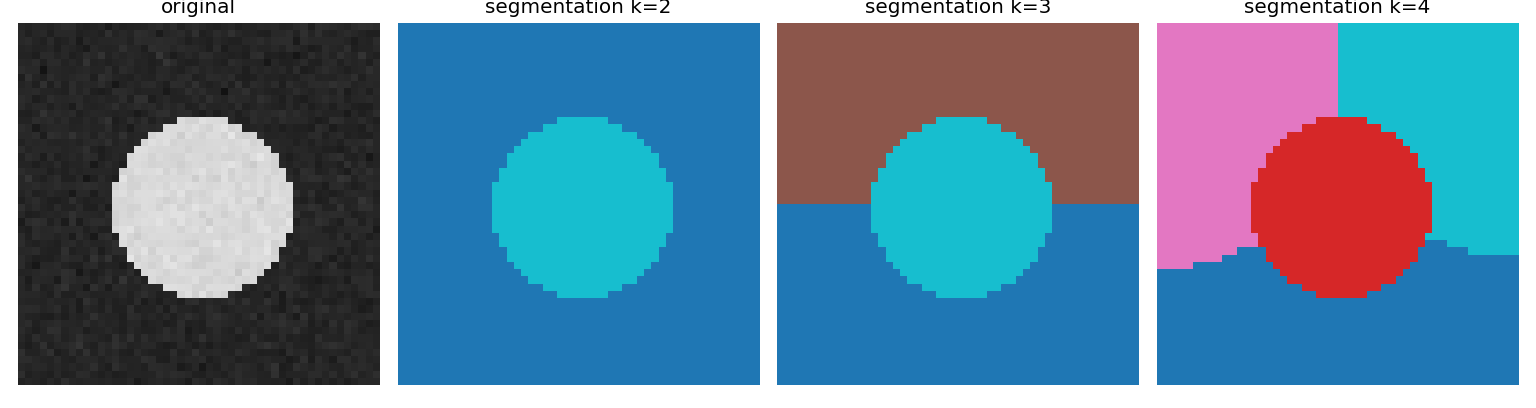
\includegraphics[width=\linewidth]{../Q4-CODE/outputs/step6_segmentation.png}\\[3pt]
{\small از چپ: تصویرِ اصلی، سپس قطعه‌بندی برای $k=2,3,4$. دیسک (خوشه‌ی $489$تایی) در هر سه ثابت می‌ماند.}
\end{center}

%==================================================================
\section{گام ۷ --- لانتساش روی تصویر بزرگِ تُنُک (پرسش ۷)}
%==================================================================

روش تا اینجا روی تصویرِ کوچکِ $50\times50$ به‌درستی کار کرد، اما برای تصاویرِ بزرگ‌تر یک محدودیتِ جدی وجود دارد: ماتریسِ $W$ متراکم برای $n=14400$ گره حدودِ دو میلیارد درایه دارد که در حافظه جای نمی‌گیرد. راهِ حل دو بخش دارد. نخست، $W$ از ابتدا به‌صورتِ \emph{تُنُک} ساخته می‌شود و تنها همسایه‌های درونِ شعاعِ $r$ ذخیره می‌شوند. دوم، از الگوریتمِ لانتساش استفاده می‌شود که هیچ‌گاه به کلِ ماتریس دسترسیِ مستقیم ندارد و تنها عملیاتش روی ماتریس، ضربِ آن در یک بردار است؛ این عملیات برای ماتریسِ تُنُک بسیار کم‌هزینه است و نیازی به ساخت، معکوس یا تجزیه‌ی ماتریس نیست. افزون بر این، چون هدف کوچک‌ترین مقادیر ویژه‌ی $L$ است ولی لانتساش بزرگ‌ترین مقادیر را سریع‌تر می‌یابد، به‌جای $L$ روی $M=2I-L$ کار می‌کنیم؛ بزرگ‌ترین مقادیر ویژه‌ی $M$ دقیقاً معادلِ کوچک‌ترین مقادیر ویژه‌ی $L$ هستند.

\begin{pycode}
\begin{lstlisting}
def lanczos(matvec, n, m, seed=0):
    q = rng.standard_normal(n); Q[:, 0] = q / np.linalg.norm(q)
    for j in range(m):
        w = matvec(Q[:, j])                       # the ONLY access to the matrix
        if j > 0: w = w - beta[j] * Q[:, j - 1]   # three-term recurrence
        alpha[j] = Q[:, j] @ w
        w = w - alpha[j] * Q[:, j]
        w = w - Q[:, :j+1] @ (Q[:, :j+1].T @ w)   # full reorthogonalization
        beta[j+1] = np.linalg.norm(w)
        if beta[j+1] < 1e-12: return alpha[:j+1], beta[1:j+1], Q[:, :j+1]
        Q[:, j+1] = w / beta[j+1]
    return alpha, beta[1:m], Q[:, :m]

def smallest_eigenvectors_lanczos(L, n_vectors, m=80, seed=0):
    matvec = lambda v: 2.0 * v - L @ v            # M = 2I - L (sparse matvec)
    alpha, beta, Q = lanczos(matvec, L.shape[0], m, seed=seed)
    T = np.diag(alpha) + np.diag(beta, 1) + np.diag(beta, -1)
    theta, S = np.linalg.eigh(T)                  # cheap: T is m x m tridiagonal
    lam = 2.0 - theta                             # back to eigenvalues of L
    order = np.argsort(lam)
    return lam[order][:n_vectors], (Q @ S[:, order])[:, :n_vectors]
\end{lstlisting}
\end{pycode}

\noindent\textbf{روندِ کد.} لانتساش گام‌به‌گام یک پایه‌ی متعامد می‌سازد و هم‌زمان ماتریسِ بزرگ را به یک ماتریسِ کوچکِ سه‌قطری فشرده می‌کند. حلقه‌ی اصلی همان رابطه‌ی بازگشتیِ سه‌جمله‌ای است: در هر گام یک ضربِ ماتریس-بردار انجام می‌شود (\file{matvec} --- تنها نقطه‌ی دسترسی به ماتریس)، سهمِ بردارِ پیشین کسر می‌شود، درایه‌ی روی قطر $\alpha_j=q_j\T w$ محاسبه و سپس باقی‌مانده نرمال می‌شود تا بردارِ بعدیِ پایه ($q_{j+1}$) به‌دست آید. خطِ \file{w = w - Q[:, :j+1] @ (Q[:, :j+1].T @ w)} بخشِ حساسِ کار است: مطابقِ تحلیلِ پرسشِ ۷، در محاسباتِ ممیزِ شناور بردارهای پایه به‌تدریج تعامدِ خود را از دست می‌دهند و مقادیر ویژه‌ی کاذب پدید می‌آید؛ این خط با متعامدسازیِ کاملِ دوباره از بروزِ چنین خطایی جلوگیری می‌کند. در پایان، ماتریسِ کوچکِ سه‌قطریِ $T_m$ باقی می‌ماند که یافتنِ مقادیر ویژه‌اش کم‌هزینه است، و چون محاسبات روی $M=2I-L$ انجام شده، با رابطه‌ی $\lambda=2-\theta$ به مقادیر ویژه‌ی $L$ بازمی‌گردیم.

\smallskip
\noindent\textbf{خروجیِ اجرا:}
\begin{consoleout}
\begin{lstlisting}
large image (120, 120) -> n = 14400, nnz(L) = 961200 (0.464% dense)
smallest eigenvalues (Lanczos): [1.896958e-08 5.164356e-04 1.444241e-03
                                  1.935965e-03 6.440775e-03]
k=4: cluster sizes = [3600, 3600, 3600, 3600]
\end{lstlisting}
\end{consoleout}

\begin{qlink}
\textbf{پرسش ۷} خواستِ استفاده از لانتساش روی ماتریسِ تُنُک بود. تصویرِ $120\times120$ یعنی $n=\mathbf{14400}$ گره، ولی $L$ فقط $\mathbf{0.464\%}$ چگال است ($961{,}200$ درایه‌ی ناصفر از $\approx2\times10^{8}$)؛ ساختِ متراکمِ آن ممکن نبود ولی لانتساشِ تُنُک به‌راحتی از پسش برمی‌آید. کوچک‌ترین مقدار ویژه $\approx\mathbf{1.9\times10^{-8}}$ (صفرِ بدیهی) و چهار مقدارِ بعدی به‌خوبی از هم جدا (گافِ طیفیِ روشن) به دست آمدند. چون تصویر عمداً چهار ربعِ متمایز دارد، $k=4$ خوشه‌های \emph{کاملاً متوازنِ} $\mathbf{[3600,3600,3600,3600]}$ داد؛ یعنی لانتساش هر چهار ناحیه را بی‌نقص و بدونِ مقدار ویژه‌ی کاذب پیدا کرد.
\end{qlink}

\begin{center}
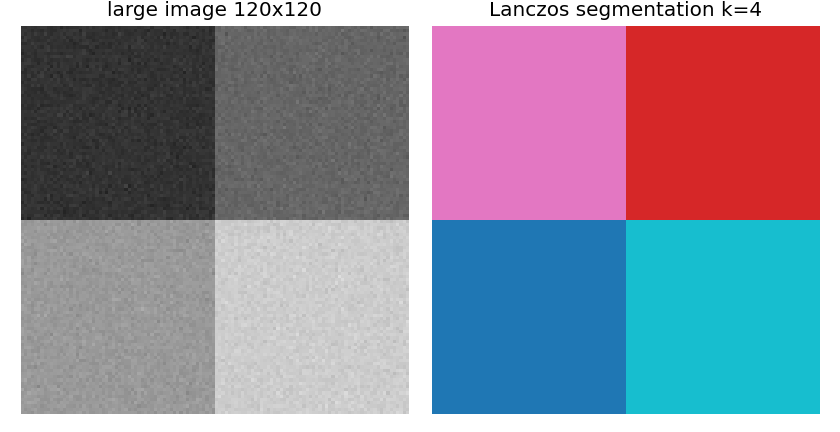
\includegraphics[width=0.78\linewidth]{../Q4-CODE/outputs/step7_lanczos.png}\\[3pt]
{\small تصویرِ بزرگِ چهارربعی و قطعه‌بندیِ کاملاً متوازنِ آن با لانتساشِ تُنُک.}
\end{center}

%==================================================================
\section{گام ۸ --- تصویر واقعیِ گورخر (مقایسه)}
%==================================================================

برای ارزیابیِ روش روی داده‌ی واقعی، همان خط‌لوله‌ی تُنُک را روی تصویرِ معروفِ گورخرِ \lr{Shi \& Malik} اجرا می‌کنیم؛ بدونِ هیچ تغییری در کد و تنها با عوض‌کردنِ ورودی. انتظارِ واقع‌بینانه این است که چون تنها ویژگیِ در دسترس روشناییِ خاکستری است (نه رنگ)، الگوریتم نواحیِ کلانِ صحنه را تفکیک کند (پیش‌زمینه از پس‌زمینه و خطِ پشتِ گورخر) و نه لزوماً یک ماسکِ دقیق از خودِ حیوان؛ این رفتار با پیش‌بینیِ گزارش سازگار است.

\noindent\textbf{خروجیِ اجرا:}
\begin{consoleout}
\begin{lstlisting}
zebra image (76, 120) -> n = 9120, nnz(L) = 1241560 (1.493% dense)
smallest eigenvalues (Lanczos): [8.881784e-16 2.417250e-03 5.060967e-03
                                  7.784443e-03 1.033946e-02]
\end{lstlisting}
\end{consoleout}

\begin{notex}
\textbf{تحلیل خروجی.} تصویرِ $76\times120$ یعنی $n=\mathbf{9120}$ و چگالیِ $L$ برابرِ $\mathbf{1.493\%}$. کوچک‌ترین مقدار ویژه $\approx0$ (بدیهی) و بقیه $[2.4,\,5.1,\,7.8,\,10.3]\times10^{-3}$ شدند. برای $k=2$ تصویر تقریباً چپ/راست تقسیم می‌شود و با افزایشِ $k$ نواحیِ زمینه و بدنه‌ی گورخر تفکیک می‌شوند؛ چون فقط روشناییِ خاکستری داریم (نه رنگ)، مرزها روی کنتراستِ روشنایی می‌افتند نه دقیقاً روی مرزِ شیء --- که رفتارِ موردانتظارِ گزارش است.
\end{notex}

\begin{center}
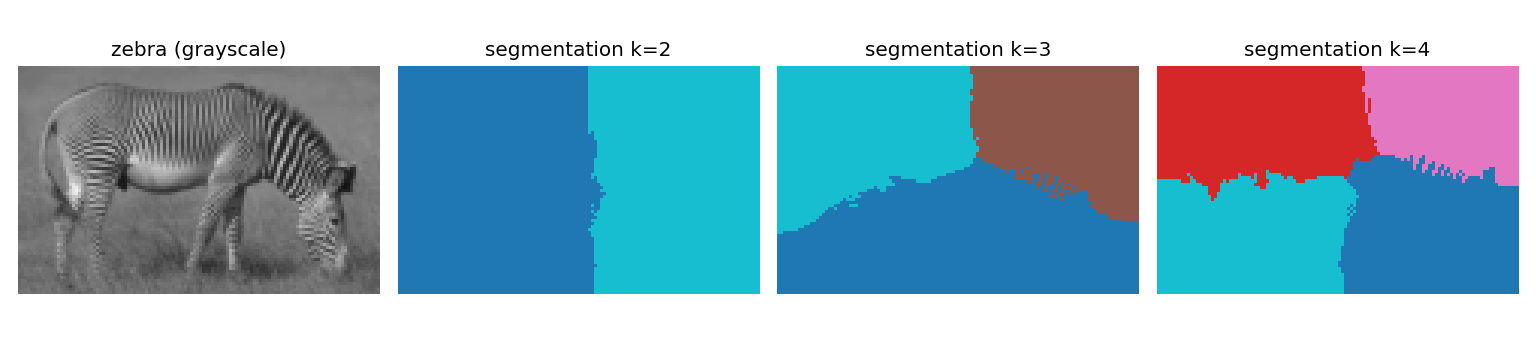
\includegraphics[width=\linewidth]{../Q4-CODE/outputs/step8_zebra.png}\\[3pt]
{\small گورخرِ خاکستری و قطعه‌بندیِ آن برای $k=2,3,4$.}
\end{center}

%==================================================================
\section{جمع‌بندی خروجی‌های عددی}
%==================================================================

\begin{center}
\renewcommand{\arraystretch}{1.35}
\arrayrulecolor{headblue!40}
\setlength{\arrayrulewidth}{0.8pt}
\begin{tabular}{|l|l|l|}
\hline
\rowcolor{headblue}
{\color{white}\textbf{پرسش}} & {\color{white}\textbf{کمیتِ عددی}} & {\color{white}\textbf{مقدار}} \\ \hline
\rowcolor{boxbg}۱-ب & تقارنِ $W$: $\norm{W-W\T}_F$ & $0.000\times10^{0}$ \\ \hline
۲-الف & تقارنِ $L$: $\norm{L-L\T}_F$ & $0.000\times10^{0}$ \\ \hline
\rowcolor{boxbg}۲-ب & بازه‌ی طیفِ $L_{\mathrm{sym}}$ & $[-3.3\times10^{-16},\,1.096]\subset[0,2]$ \\ \hline
۲-ج & باقی‌مانده‌ی بردارِ بدیهی $\norm{L\,D^{1/2}\mathbf 1}$ & $1.9\times10^{-16}$ \\ \hline
\rowcolor{boxbg}۳ & تطابقِ $\lambda_{z_3}$ با \file{eigh} & $5.152878\times10^{-3}$ (یکسان) \\ \hline
۴-الف & تعامد $|z_2\!\cdot z_1|,\ |z_3\!\cdot z_2|$ & $1.3\times10^{-16},\ 3.1\times10^{-16}$ \\ \hline
\rowcolor{boxbg}۵ & $\norm{PA-LU}$؛ $\norm{Ax-b}$ & $2.7\times10^{-16}$؛ $6.4\times10^{-16}$ \\ \hline
۶ & اندازه‌ی خوشه‌ها $k{=}2,3,4$ & $[2011,489]$؛ $[993,1018,489]$؛ $[810,489,620,581]$ \\ \hline
\rowcolor{boxbg}۷ & چگالیِ $L$؛ خوشه‌های لانتساش $k{=}4$ & $0.464\%$؛ $[3600,3600,3600,3600]$ \\ \hline
\end{tabular}
\arrayrulecolor{black}
\end{center}

\noindent همه‌ی خطاهای عددی در حدِ دقتِ ماشین ($\sim10^{-16}$) هستند و نتایجِ تصویری با تحلیلِ تئوری هم‌خوانِ کامل دارند: تقارن و کرانِ طیف رعایت می‌شود، بردارِ بدیهی درست شناسایی و حذف می‌شود، تجزیه‌ی $PLU$ و حل‌ها دقیق‌اند، و قطعه‌بندی همان رفتارِ موردانتظار (پایداریِ شیء و ریزشدنِ تدریجیِ پس‌زمینه با افزایشِ $k$) را نشان می‌دهد.

\end{document}
